
\de{ĐỀ THI HỌC KỲ II NĂM HỌC 2022-2023}{THPT Nguyễn Hữu Huân}



%Câu 1..................................
\begin{bt}%[0D7B2-2]%[0D7B3-2]%[Dự án đề kiểm tra HKII NH22-23- VUNgocHao]%[THPT Nguyễn Hữu Huân]
 Giải các phương trình, bất phương trình sau:
	\begin{enumerate}
		\item $\dfrac{x^2-5 x+4}{-x^2+4 x-4} \geq 0
		$;
		\item $\sqrt{3 x^2-2 x-6}=\sqrt{x^2+3 x+1}$.
	\end{enumerate}
	\loigiai{\begin{enumerate}
			\item
			\[\begin{aligned}
				&\dfrac{x^2-5 x+4}{-x^2+4 x-4} \geq 0\\
				\Leftrightarrow &\dfrac{x^2-5 x+4}{-(x-2)^2} \geq 0\\
				\Leftrightarrow &\heva{&x\ne 2\\&x^2-5x+4\leq 0}\\
				\Leftrightarrow &\heva{&x \ne 2 \\ &1 \leq x\leq 4.}
			\end{aligned}\]
			Vậy tập nghiệm $S=[1;4]\setminus\{2\}$.
			\item 
			\[\begin{aligned}
				&\sqrt{3 x^2-2 x-6}=\sqrt{x^2+3 x+1}\\
				\Leftrightarrow&\heva{&x^2+3x+1\geq 0\\&3x^2-2x-6=x^2+3x+1}\\
				\Leftrightarrow &\heva{&\hoac{&x\geq \dfrac{-3+\sqrt{5}}{2}\\&x\leq \dfrac{-3-\sqrt{5}}{2}}\\&2x^2-5x-7=0}\\
				\Leftrightarrow&\heva{&\hoac{&x\geq \dfrac{-3+\sqrt{5}}{2}\\&x\leq \dfrac{-3-\sqrt{5}}{2}}\\&\hoac{&x=\dfrac{7}{2}\\&x=-1}}\\
				\Leftrightarrow& x=\dfrac{7}{2}.
			\end{aligned}\]
		Vậy nghiệm của phương trình là $S=\dfrac{7}{2}.$
	\end{enumerate}}
\end{bt}

%Câu 2..................................
\begin{bt}%[0D7K2-1]%[Dự án đề kiểm tra HKII NH22-23- VUNgocHao]%[THPT Nguyễn Hữu Huân]
 Tìm tất cả các giá trị của $m$ để hàm số $f(x)=\dfrac{x-1}{\left(x^2+1\right) \sqrt{x^2-2(m+1) x+2 m+2}}$ xác định với mọi $x \in \mathbb{R}$.
	\loigiai{
		Hàm số $f(x)$ xác định với mọi $x \in \mathbb{R}$\\
		\[\begin{aligned}
		&x^2-2(m+1) x+2 m+2>0, \text{với mọi}\, x \in \mathbb{R}\\
		\Leftrightarrow &\, \Delta'=(m+1)^2-2m-2<0\\
		\Leftrightarrow &\,  m^2-1<0\\
		\Leftrightarrow &\,  -1<m<1.
	\end{aligned}\]
	Vậy $-1<m<1$ thỏa yêu cầu bài toán.	}
\end{bt}
%Câu 3..................................
\begin{bt}%[0D8B3-2]%[Dự án đề kiểm tra HKII NH22-23- VUNgocHao]%[THPT Nguyễn Hữu Huân]
 Khai triển biểu thức $\left(2 x^2+x\right)^4$ và tìm hệ số của số hạng chứa $x^5$ trong khai triển.
	\loigiai{
Công thức số hạng tổng quát của khai triển nhị thức $\left(2 x^2+x\right)^4$ là 
	\[\begin{aligned}
	 T_{k+1} & = \mathrm{C}_{4}^{k}\cdot(2x^2)^{4-k}\cdot x^{k}\\
	 = &  \mathrm{C}_{4}^{k}\cdot2^{4-k}\cdot x^{8-2k}\cdot x^k\\
	 = & \mathrm{C}_{4}^{k}\cdot2^{4-k}\cdot x^{8-k}.
\end{aligned}\]
Cho $8-k =5 \Leftrightarrow k = 3$. \\
Khi đó hệ số của số hạng chứa $x^5$ trong khai triển là $\mathrm{C}_4^3\cdot2^{4-3}=8$.
}
\end{bt}
%Câu 4..................................
\begin{bt}%%[0D8K2-1]%[Dự án đề kiểm tra HKII NH22-23- VUNgocHao]%[THPT Nguyễn Hữu Huân]
 Tổ Một có có $7$ học sinh nam, $5$ học sinh nữ. Hỏi có bao nhiêu cách chọn ra $3$ học sinh từ tổ Một đi dự đại hội, biết rằng $3$ học sinh được chọn có cả nam và nữ?
	\loigiai{
	\begin{itemize}
		\item 	TH1: $3$ học sinh được chọn có $1$ nam và $2$ nữ:\\
		+ Chọn $1$ học sinh nam từ $7$ học sinh nam có $\mathrm{C}_7^1 = 7$ cách.\\
		+ Chọn $2$ học sinh nữ từ $5$ học sinh nữ có $\mathrm{C}_5^2 = 10$ cách.\\
		Do đó có $7\cdot 10=70$ cách.\\
		\item TH2: $3$ học sinh được chọn có $2$ nam và $1$ nữ:\\
		+ Chọn $2$ học sinh nam từ $7$ học sinh nam có $C_7^2 = 21$ cách.\\
		+ Chọn $1$ học sinh nữ từ $5$ học sinh nữ có $\mathrm{C}_5^1 = 5$ cách.\\
		Do đó có $21\cdot 5=105$ cách.
	\end{itemize}
	Suy ra số cách chọn $3$ học sinh có cả nam và nữ là $70 + 105 =175$ cách.
}
\end{bt}
%Câu 5..................................
\begin{bt}%[0D8G2-2]%[Dự án đề kiểm tra HKII NH22-23- VUNgocHao]%[THPT Nguyễn Hữu Huân]
 Có bao nhiêu cách xếp ngẫu nhiên $8$ học sinh gồm $4$ học sinh nam (trong đó có Việt) và $4$ học sinh nữ (trong đó có An) thành một hàng ngang sao cho trong $8$ học sinh trên không có hai học sinh cùng giới đứng cạnh nhau, đồng thời Việt và An cũng không đứng cạnh nhau?
	\loigiai{
	Ta đánh số hàng ngang từ $1$ đến $8$.
	\begin{itemize}
		\item 	TH1: Nam xếp vị trí lẻ, nữ xếp vị trí chẵn:
		\begin{itemize}
			\item Việt đứng đầu hàng\\
			+ Việt xếp vị trí số $1$ có $1$ cách.\\
			+ Xếp $3$ nam còn lại vào các vị trí $3, 5, 7$ có $3!$ cách.\\
			+ Vì Việt và An không đứng cạch nhau nên An có thể xếp ở các vị trí $4, 6, 8$. Do đó xếp An có $3$ cách.\\
			+ Xếp $3$ nữ vào các vị trí còn lại có $3!$ cách.\\
			Do đó số cách xếp là $1\cdot3!\cdot3\cdot3!= 108$. cách.
			\item Việt đứng giữa hàng\\
			+ Xếp Việt vào một trong ba vị trí $3, 5, 7$ có $3$ cách.\\
			+ Xếp $3$ nam vào các vị trí còn lại có $3!$ cách.\\
			+ Vì An và Việt không đứng cạnh nhau nên xếp An có $2$ cách.\\
			+ Xếp $3$ nữ vào $3$ vị trí còn lại có $3!$ cách.\\
			Do đó số cách xếp là $3\cdot 3!\cdot2\cdot 3!=216$ cách.
		\end{itemize}
		Số cách xếp TH1 là $108 + 216 =324$ cách.
		\item 	TH2: Nữ xếp vị trí lẻ, nam xếp vị trí chẵn.\\
		Lập luận tương tự, ta có số cách xếp TH2 là $324$ cách.
		\end{itemize}
		Vậy số cách xếp thỏa mãn yêu cầu bài toán là $324 + 324 = 648$ cách.



}
\end{bt}

\begin{bt}%[0T9B3-2]%[Dự án đề kiểm tra HKII NH22-23- Lương Như Quỳnh]%[Trường THPT Nguyễn Hữu Huân]
	Trong mặt phẳng $Oxy$, cho tam giác $ABC$ với $A(4;0)$, $B(-3;7)$, $C(-10;0)$ và đường thẳng $d\colon 3x-2y+1=0$.
	\begin{enumerate}
		\item Viết phương trình đường tròn $(C)$ ngoại tiếp tam giác $ABC$.
		\item Tìm số nguyên $k$ sao cho đường thẳng $\Delta \colon x+ky-1-2k=0$ tạo với đường thẳng $d$ một góc $45^{\circ}$.
	\end{enumerate}
\loigiai{
	\begin{enumerate}
		\item Phương trình đường tròn $(C)$ có dạng $ x^2+y^2-2ax-2by+c=0$ ($ a^2+b^2-c>0 $).\\
		Ta có $A$, $B$, $ C\in (C) $ suy ra
		\[\heva{&16+0-8a+c=0\\&9+49+6a-14b+c=0\\&100+20a+c=0}\Leftrightarrow \heva{&a=-3\\&b=0\\&c=-40.}\]
		Vậy $(C)\colon x^2+y^2+6x-40=0$.
		\item Đường thẳng $\Delta$ có một véc-tơ pháp tuyến là $ \overrightarrow{n_{\Delta}}=(1;k)$.\\
		Đường thẳng $d$ có một véc-tơ pháp tuyến là $ \overrightarrow{n_d}=(3;-2)$.\\
		Ta có 
		\allowdisplaybreaks
		\begin{eqnarray*}
		 && \cos 45^\circ =\cos (\Delta,d) =\dfrac{\left|1\cdot 3+k(-2)\right|}{\sqrt{1^2+k^2}\cdot \sqrt{3^2+(-2)^2}} \\ 
  		&\Leftrightarrow& 2(3-2k)^2=13\left(1+k^2\right)\Leftrightarrow 5k^2+24k-5=0\\ 
  		&\Leftrightarrow& \hoac{&k=\dfrac{1}{5}\\&k=-5.} \\ 
		\end{eqnarray*}
Vì $ k $ nguyên nên $ k=-5 $.
	\end{enumerate}
}
\end{bt}

\begin{bt}%[0T9B4-5]%[Dự án đề kiểm tra HKII NH22-23- Lương Như Quỳnh]%[Trường THPT Nguyễn Hữu Huân]
	Viết phương trình chính tắc của Hyperbol $(H)$, biết $(H)$ có một tiêu điểm $F_2(5;0)$ và độ dài trục thực bằng $8$.
\loigiai{
Phương trình chính tắc của hyperbol $(H)$ có dạng
$ \dfrac{x^2}{a^2}-\dfrac{y^2}{b^2}=1 $, ($ a>b>0 $).\\
$(H)$ có một tiêu điểm $F_2(5;0)$ suy ra $ c=5 $.\\
$(H)$ có độ dài trục thực bằng $8$ suy ra $ 2a=8\Leftrightarrow a=4 $.\\
Ta có $ b=\sqrt{c^2-a^2} =\sqrt{5^2-4^2}=3$.\\
Vậy $(H)\colon \dfrac{x^2}{16}-\dfrac{y^2}{9}=1$.
}
\end{bt}

\begin{bt}%[0T9T4-0]%[Dự án đề kiểm tra HKII NH22-23- Lương Như Quỳnh]%[Trường THPT Nguyễn Hữu Huân]
	Hình vẽ sau đây minh họa một căn phòng thì thầm (whispering gallery) với mặt cắt ngang là một hình bán elip cao $7$ mét và rộng $30$ mét. Căn phòng này có đặc điểm: Nếu một người đứng ở một tiêu điểm của phòng thì có thể nghe thấy âm thanh phát ra từ một người khác đứng ở tiêu điểm còn lại (dù âm thanh đó rất nhỏ).
	\definecolor{tumbleweed}{rgb}{0.87, 0.67, 0.53}%màu da	
	\definecolor{ballblue}{rgb}{0.13, 0.67, 0.8}
	\definecolor{dimgray}{rgb}{0.41, 0.41, 0.41}
	\definecolor{darkbrown}{rgb}{0.4, 0.26, 0.13}
	\definecolor{darkcoral}{rgb}{0.8, 0.36, 0.27}
	\definecolor{darkcandyapplered}{rgb}{0.64, 0.0, 0.0}
	\definecolor{burlywood}{rgb}{0.87, 0.72, 0.53}
\begin{center}
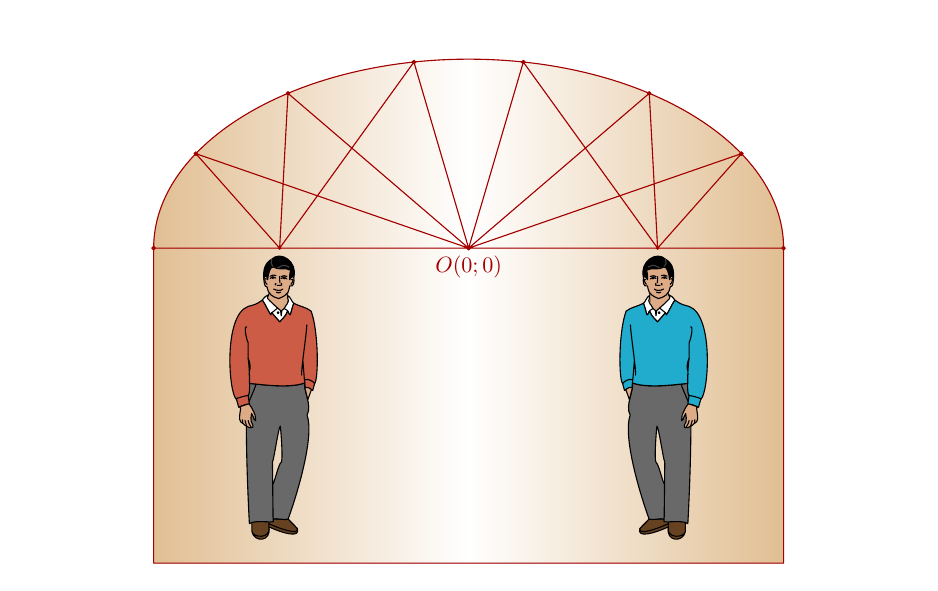
\begin{tikzpicture}[line join=round, line cap=round,scale=.8,transform shape]
\clip (-7,-5) rectangle (7,3.5);

\tikzset{man_2/.pic={
\def\T{ 
(-.25,4.45)%điểm rẽ ngôi 1
..controls +(-150:.3) and +(95:.25) .. (-.5,3.8) %vành tai trái
..controls +(85:.2) and +(95:.1) .. (-.38,3.8)%vành tai 2
..controls +(85:.2) and +(160:.1) .. (-.2,4.2)%điểm rẽ ngôi phải
..controls +(-35:.2) and +(150:.2) .. (.35,4.1)
..controls +(-105:.2) and +(85:.1) .. (.32,3.8)
..controls +(65:.1) and +(115:.05) .. (.45,3.88)
..controls +(75:.5) and +(45:.4) .. cycle
;}
\draw \T;
\fill \T;
\draw[darkgray] (-.25,4.45)%điểm rẽ ngôi 1
..controls +(-120:.1) and +(140:.1) .. (-.2,4.2) %điểm rẽ ngôi 2
(-.1,4.15)
..controls +(30:.2) and +(150:.2) .. (.3,4.2)
;
%---------------------------
\def\C{ %cổ
%cổ
(-.33,3.38)
..controls +(-110:.1) and +(50:.05) .. (-.38,3.2)
..controls +(-50:.1) and +(150:.05) .. (.03,2.82)--(.05,2.68)--(.07,2.82)
..controls +(30:.12) and +(-150:.05) .. (.24,3.03)
..controls +(110:.1) and +(95:.05) .. (.26,3.38)
;
}
\draw \C;
\fill[tumbleweed] \C;
%---------------------------giày
\def\G{
(.27,-3.8)%chân quần phải
..controls +(-50:.1) and +(130:.1) .. (.56,-4.1)
..controls +(-70:.35) and +(-25:.45) .. (-.34,-4.05)--(-.34,-3.8)--cycle
(-.34,-4.05)--(-.34,-3.8)--(-.88,-3.8)--(-.88,-4.2)
..controls +(-80:.35) and +(-80:.5) ..cycle
(-.88,-4.2)
..controls +(-80:.2) and +(-80:.4) ..(-.34,-4.05)
;
}
\fill[darkbrown] \G;
\draw \G;
\draw (.56,-4.1)
..controls +(-70:.25) and +(-25:.35) .. (-.34,-3.95);
%---------------------------quần
\def\Q{
(-.96,.5)%chân áo trái
..controls +(10:.1) and +(-160:.6) .. (.8,.52)%chân áo phải
..controls +(-110:.2) and +(60:.35) .. (.87,-.5)
..controls +(-70:.7) and +(70:.9) .. (.27,-3.8)%chân quần phải
..controls +(-150:.1) and +(20:.1) .. (-.2,-3.8)
..controls +(110:.1) and +(-80:.1) .. (-.22,-2.7)
..controls +(50:.1) and +(-150:.1) .. (.05,-2)
..controls +(50:.1) and +(-80:.1) .. (0.02,-.85)
..controls +(-130:.1) and +(60:.1) .. (-.23,-2)
..controls +(-85:.1) and +(100:.1) .. (-.2,-3.88)
..controls +(-155:.1) and +(40:.2) .. (-.96,-3.95)
..controls +(95:.1) and +(-115:.5) .. cycle
;
}
\fill[dimgray] \Q;
\draw \Q;
%\draw (0.02,-.85)..controls +(50:.1) and +(-80:.1) .. (0.04,-.32);
\draw (-.75,.5)..controls +(50:.1) and +(-80:.1) .. (-1.2,-.5);
%---------------------------
\def\C1{ %cổ áo
(-.34,3.33)
..controls +(-120:.1) and +(110:.05) .. (-.38,3.2)
..controls +(-50:.1) and +(150:.05) .. (.03,2.82)--(.05,2.65)--(.07,2.82)
..controls +(30:.12) and +(-150:.05) .. (.24,3.03)
..controls +(50:.1) and +(-65:.05) .. (.26,3.2)--(.25,3.3)
..controls +(-20:.1) and +(160:.06) .. (.45,3.05)%vai phải
..controls +(-110:.1) and +(85:.06) .. (.35,2.7)
..controls +(-110:.1) and +(85:.06) .. (.25,2.8)
..controls +(-110:.15) and +(45:.2) .. (0,2.46)%điểm tim áo
..controls +(125:.17) and +(-55:.2) .. (-.25,2.75)--(-.28,2.68)
..controls +(125:.17) and +(-55:.2) .. (-.55,3.15)%vai trái
..controls +(55:.12) and +(-155:.1) .. cycle
;
}
\fill[white] \C1;
\draw \C1;
\draw (-.25,2.75)
..controls +(35:.12) and +(-150:.05) .. (-.06,2.9)
(.25,2.82)
..controls +(135:.07) and +(-30:.07) .. (.15,2.88);
%-----------------------------
\def\A{
%áo
(.45,3.05)%vai phải
..controls +(-110:.1) and +(85:.06) .. (.35,2.7)
..controls +(-110:.1) and +(85:.06) .. (.25,2.8)
..controls +(-110:.15) and +(45:.2) .. (0,2.46)%điểm tim áo
..controls +(125:.17) and +(-55:.2) .. (-.25,2.75)--(-.28,2.68)
..controls +(125:.17) and +(-55:.2) .. (-.55,3.15)%vai trái
..controls +(-145:.25) and +(15:.2) .. (-1,2.95)
..controls +(-160:.85) and +(145:.3) .. (-1.37,0)--(-1.3,-.25)%tay trái
..controls +(20:.1) and +(165:.1) .. (-.96,-.16)--(-1,.12)
..controls +(20:.1) and +(-75:.1) .. (-1,1.3)
..controls +(-60:.1) and +(60:.1) .. (-.96,.9)
..controls +(-100:.1) and +(80:.1) .. (-.96,.5)%chân áo trái
..controls +(10:.1) and +(-160:.6) .. (.8,.52)%chân áo phải
--(.81,.38)
..controls +(10:.1) and +(150:.1) .. (1.05,.28)--(1.11,.5)
..controls +(50:.2) and +(-70:.7) .. (1,2.8)%vai phải
..controls +(140:.2) and +(-30:.2) .. cycle
;
}
\fill[ballblue] \A;
\draw \A;

\draw (-1,.12)
..controls +(20:.1) and +(165:.1) ..  (-1.37,0)
(-1,1.3)--(-1,1.8)
..controls +(120:.1) and +(165:.1) ..  (-1.05,2.3)
(1.11,.5)
..controls +(120:.1) and +(25:.1) .. (.8,.62)
(.8,.52)
..controls +(100:.1) and +(-85:.1) .. (.74,1.2)
(.7,.77)
..controls +(100:.15) and +(-85:.15) .. (.86,2.36)
;
%-------------------------------
\def\K{ %khuôn mặt
(-.5,3.8) %vành tai trái
..controls +(85:.2) and +(95:.1) .. (-.38,3.8)%vành tai 2
..controls +(85:.2) and +(160:.1) .. (-.2,4.2)%điểm rẽ ngôi phải
..controls +(-35:.2) and +(150:.2) .. (.35,4.1)
..controls +(-105:.2) and +(85:.1) .. (.32,3.8)
..controls +(65:.1) and +(115:.05) .. (.45,3.88)
..controls +(-85:.15) and +(-15:.15) .. (.32,3.6)
..controls +(-110:.1) and +(20:.4) .. (-.03,3.2)
..controls +(165:.2) and +(-80:.25) .. (-.4,3.57)
..controls +(120:.06) and +(-85:.3) .. cycle
%tay
(-1.3,-.25)%tay trái
..controls +(30:.2) and +(165:.25) .. (-1.17,-.76)
..controls +(-40:.15) and +(155:.1) .. (-1.05,-.85)
..controls +(-40:.1) and +(175:.05) .. (-.9,-.9)
..controls +(-10:.11) and +(-55:.05) .. (-.9,-.72)
..controls +(110:.1) and +(-95:.1) .. (-.89,-.45)--(-.84,-.55)
..controls +(-70:.05) and +(-175:.05) .. (-.76,-.68)--(-.78,-.5)
..controls +(110:.15) and +(-45:.1) .. (-.98,-.14)--cycle
%tay phải
(.81,.38)
..controls +(10:.1) and +(150:.1) .. (1.01,.31)
..controls +(-110:.5) and +(55:.05) .. (.89,0)--(.8,.38)
;
}
\fill[tumbleweed] \K;
\draw (-1.18,-.76)--(-1.18,-.65)
(-1.05,-.85)--(-1.1,-.67)
(-.9,-.89) ..controls +(140:.1) and +(-65:.05) .. (-1,-.67)
;  %ngón tay

\draw \K;
%----------------------------------
\def\M{ %các nét mặt
(-.42,3.82)
..controls +(140:.11) and +(145:.1) .. (-.4,3.65)%vành tai trong trái
(.38,3.8) %vành tai trong phải
..controls +(35:.1) and +(50:.1) .. (.36,3.65)
(-.3,3.91) %chân mày 1
..controls +(45:.06) and +(150:.05) .. (-.12,3.93)
(.05,3.9) %chân mày 2
..controls +(45:.06) and +(150:.05) .. (.23,3.9)
(-.3,3.84) %mắt trái
..controls +(45:.09) and +(140:.09) .. (-.13,3.85)
(.05,3.84) %mắt phải
..controls +(45:.09) and +(140:.09) .. (.23,3.82)
(0,3.9) %mũi
..controls +(-100:.05) and +(95:.05) .. (0.01,3.7)
(-.12,3.68) %cánh mũi trái
..controls +(-150:.03) and +(150:.03) .. (-.13,3.63)
(.06,3.68) %cánh mũi phải
..controls +(-50:.03) and +(50:.03) .. (.06,3.62)
(-.08,3.62) 
..controls +(-30:.05) and +(-150:.05) .. (.03,3.62)
(-.19,3.5) 
..controls +(-30:.1) and +(-130:.08) .. (.1,3.5)
(-.1,3.4) 
..controls +(-30:.05) and +(-150:.05) .. (.03,3.4)
;
\draw[fill=black] (.14,3.85) circle(.65pt);%con ngươi
\draw[fill=white] (.16,3.85) circle(.5pt);
\draw[fill=black] (-.22,3.86) circle(.66pt);
\draw[fill=white] (-.21,3.86) circle(.5pt);
\draw[fill=white] (-.05,2.75) circle(.8pt);%nút áo
}
\draw \M;
%\fill \M;
}}

\tikzset{man/.pic={
\def\T{ 
(-.25,4.45)%điểm rẽ ngôi 1
..controls +(-150:.3) and +(95:.25) .. (-.5,3.8) %vành tai trái
..controls +(85:.2) and +(95:.1) .. (-.38,3.8)%vành tai 2
..controls +(85:.2) and +(160:.1) .. (-.2,4.2)%điểm rẽ ngôi phải
..controls +(-35:.2) and +(150:.2) .. (.35,4.1)
..controls +(-105:.2) and +(85:.1) .. (.32,3.8)
..controls +(65:.1) and +(115:.05) .. (.45,3.88)
..controls +(75:.5) and +(45:.4) .. cycle
;}
\draw \T;
\fill \T;
\draw[darkgray] (-.25,4.45)%điểm rẽ ngôi 1
..controls +(-120:.1) and +(140:.1) .. (-.2,4.2) %điểm rẽ ngôi 2
(-.1,4.15)
..controls +(30:.2) and +(150:.2) .. (.3,4.2)
;
%---------------------------
\def\C{ %cổ
%cổ
(-.33,3.38)
..controls +(-110:.1) and +(50:.05) .. (-.38,3.2)
..controls +(-50:.1) and +(150:.05) .. (.03,2.82)--(.05,2.68)--(.07,2.82)
..controls +(30:.12) and +(-150:.05) .. (.24,3.03)
..controls +(110:.1) and +(95:.05) .. (.26,3.38)
;
}
\draw \C;
\fill[tumbleweed] \C;
%---------------------------giày
\def\G{
(.27,-3.8)%chân quần phải
..controls +(-50:.1) and +(130:.1) .. (.56,-4.1)
..controls +(-70:.35) and +(-25:.45) .. (-.34,-4.05)--(-.34,-3.8)--cycle
(-.34,-4.05)--(-.34,-3.8)--(-.88,-3.8)--(-.88,-4.2)
..controls +(-80:.35) and +(-80:.5) ..cycle
(-.88,-4.2)
..controls +(-80:.2) and +(-80:.4) ..(-.34,-4.05)
;
}
\fill[darkbrown] \G;
\draw \G;
\draw (.56,-4.1)
..controls +(-70:.25) and +(-25:.35) .. (-.34,-3.95);
%---------------------------quần
\def\Q{
(-.96,.5)%chân áo trái
..controls +(10:.1) and +(-160:.6) .. (.8,.52)%chân áo phải
..controls +(-110:.2) and +(60:.35) .. (.87,-.5)
..controls +(-70:.7) and +(70:.9) .. (.27,-3.8)%chân quần phải
..controls +(-150:.1) and +(20:.1) .. (-.2,-3.8)
..controls +(110:.1) and +(-80:.1) .. (-.22,-2.7)
..controls +(50:.1) and +(-150:.1) .. (.05,-2)
..controls +(50:.1) and +(-80:.1) .. (0.02,-.85)
..controls +(-130:.1) and +(60:.1) .. (-.23,-2)
..controls +(-85:.1) and +(100:.1) .. (-.2,-3.88)
..controls +(-155:.1) and +(40:.2) .. (-.96,-3.95)
..controls +(95:.1) and +(-115:.5) .. cycle
;
}
\fill[dimgray] \Q;
\draw \Q;
%\draw (0.02,-.85)..controls +(50:.1) and +(-80:.1) .. (0.04,-.32);
\draw (-.75,.5)..controls +(50:.1) and +(-80:.1) .. (-1.2,-.5);

%---------------------------
\def\C1{ %cổ áo
(-.34,3.33)
..controls +(-120:.1) and +(110:.05) .. (-.38,3.2)
..controls +(-50:.1) and +(150:.05) .. (.03,2.82)--(.05,2.65)--(.07,2.82)
..controls +(30:.12) and +(-150:.05) .. (.24,3.03)
..controls +(50:.1) and +(-65:.05) .. (.26,3.2)--(.25,3.3)
..controls +(-20:.1) and +(160:.06) .. (.45,3.05)%vai phải
..controls +(-110:.1) and +(85:.06) .. (.35,2.7)
..controls +(-110:.1) and +(85:.06) .. (.25,2.8)
..controls +(-110:.15) and +(45:.2) .. (0,2.46)%điểm tim áo
..controls +(125:.17) and +(-55:.2) .. (-.25,2.75)--(-.28,2.68)
..controls +(125:.17) and +(-55:.2) .. (-.55,3.15)%vai trái
..controls +(55:.12) and +(-155:.1) .. cycle
;
}
\fill[white] \C1;
\draw \C1;
\draw (-.25,2.75)
..controls +(35:.12) and +(-150:.05) .. (-.06,2.9)
(.25,2.82)
..controls +(135:.07) and +(-30:.07) .. (.15,2.88);
%-----------------------------
\def\A{
%áo
(.45,3.05)%vai phải
..controls +(-110:.1) and +(85:.06) .. (.35,2.7)
..controls +(-110:.1) and +(85:.06) .. (.25,2.8)
..controls +(-110:.15) and +(45:.2) .. (0,2.46)%điểm tim áo
..controls +(125:.17) and +(-55:.2) .. (-.25,2.75)--(-.28,2.68)
..controls +(125:.17) and +(-55:.2) .. (-.55,3.15)%vai trái
..controls +(-145:.25) and +(15:.2) .. (-1,2.95)
..controls +(-160:.85) and +(145:.3) .. (-1.37,0)--(-1.3,-.25)%tay trái
..controls +(20:.1) and +(165:.1) .. (-.96,-.16)--(-1,.12)
..controls +(20:.1) and +(-75:.1) .. (-1,1.3)
..controls +(-60:.1) and +(60:.1) .. (-.96,.9)
..controls +(-100:.1) and +(80:.1) .. (-.96,.5)%chân áo trái
..controls +(10:.1) and +(-160:.6) .. (.8,.52)%chân áo phải
--(.81,.38)
..controls +(10:.1) and +(150:.1) .. (1.05,.28)--(1.11,.5)
..controls +(50:.2) and +(-70:.7) .. (1,2.8)%vai phải
..controls +(140:.2) and +(-30:.2) .. cycle
;
}
\fill[darkcoral] \A;
\draw \A;
\draw (-1,.12)
..controls +(20:.1) and +(165:.1) ..  (-1.37,0)
(-1,1.3)--(-1,1.8)
..controls +(120:.1) and +(165:.1) ..  (-1.05,2.3)
(1.11,.5)
..controls +(120:.1) and +(25:.1) .. (.8,.62)
(.8,.52)
..controls +(100:.1) and +(-85:.1) .. (.74,1.2)
(.7,.77)
..controls +(100:.15) and +(-85:.15) .. (.86,2.36)
;
%-------------------------------
\def\K{ %khuôn mặt
(-.5,3.8) %vành tai trái
..controls +(85:.2) and +(95:.1) .. (-.38,3.8)%vành tai 2
..controls +(85:.2) and +(160:.1) .. (-.2,4.2)%điểm rẽ ngôi phải
..controls +(-35:.2) and +(150:.2) .. (.35,4.1)
..controls +(-105:.2) and +(85:.1) .. (.32,3.8)
..controls +(65:.1) and +(115:.05) .. (.45,3.88)
..controls +(-85:.15) and +(-15:.15) .. (.32,3.6)
..controls +(-110:.1) and +(20:.4) .. (-.03,3.2)
..controls +(165:.2) and +(-80:.25) .. (-.4,3.57)
..controls +(120:.06) and +(-85:.3) .. cycle
%tay
(-1.3,-.25)%tay trái
..controls +(30:.2) and +(165:.25) .. (-1.17,-.76)
..controls +(-40:.15) and +(155:.1) .. (-1.05,-.85)
..controls +(-40:.1) and +(175:.05) .. (-.9,-.9)
..controls +(-10:.11) and +(-55:.05) .. (-.9,-.72)
..controls +(110:.1) and +(-95:.1) .. (-.89,-.45)--(-.84,-.55)
..controls +(-70:.05) and +(-175:.05) .. (-.76,-.68)--(-.78,-.5)
..controls +(110:.15) and +(-45:.1) .. (-.98,-.14)--cycle
%tay phải
(.81,.38)
..controls +(10:.1) and +(150:.1) .. (1.01,.31)
..controls +(-110:.5) and +(55:.05) .. (.89,0)--(.8,.38)
;
}
\fill[tumbleweed] \K;
\draw (-1.18,-.76)--(-1.18,-.65)
(-1.05,-.85)--(-1.1,-.67)
(-.9,-.89) ..controls +(140:.1) and +(-65:.05) .. (-1,-.67)
;  %ngón tay
\draw \K;
%----------------------------------
\def\M{ %các nét mặt
(-.42,3.82)
..controls +(140:.11) and +(145:.1) .. (-.4,3.65)%vành tai trong trái
(.38,3.8) %vành tai trong phải
..controls +(35:.1) and +(50:.1) .. (.36,3.65)
(-.3,3.91) %chân mày 1
..controls +(45:.06) and +(150:.05) .. (-.12,3.93)
(.05,3.9) %chân mày 2
..controls +(45:.06) and +(150:.05) .. (.23,3.9)
(-.3,3.84) %mắt trái
..controls +(45:.09) and +(140:.09) .. (-.13,3.85)
(.05,3.84) %mắt phải
..controls +(45:.09) and +(140:.09) .. (.23,3.82)
(0,3.9) %mũi
..controls +(-100:.05) and +(95:.05) .. (0.01,3.7)
(-.12,3.68) %cánh mũi trái
..controls +(-150:.03) and +(150:.03) .. (-.13,3.63)
(.06,3.68) %cánh mũi phải
..controls +(-50:.03) and +(50:.03) .. (.06,3.62)
(-.08,3.62) 
..controls +(-30:.05) and +(-150:.05) .. (.03,3.62)
(-.19,3.5) 
..controls +(-30:.1) and +(-130:.08) .. (.1,3.5)
(-.1,3.4) 
..controls +(-30:.05) and +(-150:.05) .. (.03,3.4)
;
\draw[fill=black] (.14,3.85) circle(.65pt);%con ngươi
\draw[fill=white] (.16,3.85) circle(.5pt);
\draw[fill=black] (-.22,3.86) circle(.66pt);
\draw[fill=white] (-.21,3.86) circle(.5pt);
\draw[fill=white] (-.05,2.75) circle(.8pt);%nút áo
}
\draw \M;
%\fill \M;
}}
\fill[left color=burlywood!90,right color=burlywood!90, middle color=white]
(5,0) arc (0:180:5 cm and 3cm)--(-5,-5)--(5,-5)--cycle;
\draw[darkcandyapplered] (5,0) arc (0:180:5 cm and 3cm)--(-5,-5)--(5,-5)--cycle;
\draw[darkcandyapplered,fill=darkcandyapplered]
(3,0)--(30:5 cm and 3cm)circle(.8pt)--(0,0)
(3,0)--(55:5 cm and 3cm)circle(.8pt)--(0,0)
(3,0)--(80:5 cm and 3cm)circle(.8pt)--(0,0)
(-3,0)--(100:5 cm and 3cm)circle(.8pt)--(0,0)
(-3,0)--(125:5 cm and 3cm)circle(.8pt)--(0,0)
(-3,0)--(150:5 cm and 3cm)circle(.8pt)--(0,0)
(-5,0)circle(.8pt)--(5,0)circle(.8pt)
(0,0)circle(.8pt)
;
\node[darkcandyapplered] at (0,0) [below]{$O(0;0)$};
\fill[darkcandyapplered] (-3,0) circle(.8pt);
\fill[darkcandyapplered] (3,0) circle(.8pt);
\path 
(-3,-2.4)pic[scale=.5]{man}
(3,-2.4)pic[scale=.5,rotate=180,yscale=-1]{man_2}
;
\end{tikzpicture}
\end{center}
	\begin{enumerate}
		\item Để hai người có thể \lq\lq nói thì thầm với nhau\rq\rq\, trong căn phòng này thì mỗi người cần đúng cách trung tâm của phòng xấp xỉ bao nhiêu mét?
		\item Giả sử âm thanh \lq\lq thì thầm\rq\rq\, từ một người đứng ở một tiêu điểm của phòng sau khi đến một điểm trên trần vòm elip sẽ cho tia phản xạ đến người đứng ở tiêu điểm còn lại. Hỏi sau bao nhiêu giây người còn lại sẽ nghe được âm thanh đó? Biết vận tốc âm thanh là $343{,}2$ mét/giây.
	\end{enumerate}
\textit{(Làm tròn kết quả đến một chữ số thập phân sau dấu phẩy.)}
\loigiai{
\begin{enumerate}
\item Mặt cắt ngang căn phòng là một hình bán elip cao $7$ mét và rộng $30$ mét suy ra \[b=7,\,a=\dfrac{30}{2}=15 .\]
Để hai người có thể \lq\lq nói thì thầm với nhau\rq\rq\, trong căn phòng này thì mỗi người cần đứng cách trung tâm của phòng một nửa tiêu cự là \[ c=\sqrt{a^2-b^2}=\sqrt{15^2-7^2}=4\sqrt{11}\approx 13{,}3 \text{ mét.}\]
		\item Quãng đường đi của âm thanh là $ S=2a=30 $ mét. \\
		Thời gian âm thanh đi là $ t=\dfrac{S}{v}=\dfrac{30}{343{,}2} \approx 0{,}1$ giây.\\
		Vậy sau $0{,}1$ giây người còn lại sẽ nghe được âm thanh đó.
\end{enumerate}
}
\end{bt}




